\documentclass[12pt,a4paper]{report}

%---------- packages imports --------

\usepackage[english]{babel}		% makes english syllabization for breaking words between lines
\usepackage{xspace}				% adds a space between words when used a custom command
%\usepackage{indentfirst}		% indents the first line of the first paragraph of a section
%\usepackage{enumitem}			% to create custom enumerations
%\usepackage{clipboard}			% to copy-paste a certain piece of text in several parts of the doc
\usepackage{tabularx}			% to create tables that do automatic line break of the text inside
\usepackage{graphicx}			% for including images
	\graphicspath{{./images/}}
	
%\usepackage{subcaption}			% multiple figures
%\usepackage{scrextend}			% for text indentation	

\usepackage[dvipsnames]{xcolor}	% color in text
\usepackage{listings}			% code snippets
\lstset{
	language=Octave,
	frame=l,						% left line
	tabsize=2,						% tab indentation
	belowskip=1em,					% space after code
	basicstyle=\linespread{0.9}\ttfamily		% line space
}

%\usepackage[export]{adjustbox}	% add border to figures

\usepackage{amsmath}					% matrix environment
\setlength\arraycolsep{8pt}				% matrix horizontal spacing

\usepackage[braket, qm]{qcircuit}

\usepackage{tikz}
\usetikzlibrary{calc}

\usepackage[nodisplayskipstretch]{setspace} \setstretch{1.5}

\usepackage[hidelinks]{hyperref}	% to have clickable URLs, hidelinks is for removing visible boxes in links (should be the last package, before cleveref)
\usepackage[capitalise, noabbrev]{cleveref}	% to put the word 'Figure' before the number

\newcommand{\tikzmark}[1]{\tikz[overlay,remember picture] \node (#1) {};}
\newcommand{\DrawBox}[4][]{%
	\tikz[overlay,remember picture]{%
		\coordinate (TopLeft)     at ($(#2)+(-0.1em,0.9em)$);
		\coordinate (BottomRight) at ($(#3)+(0.1em,-0.3em)$);
		%
		\path (TopLeft); \pgfgetlastxy{\XCoord}{\IgnoreCoord};
		\path (BottomRight); \pgfgetlastxy{\IgnoreCoord}{\YCoord};
		\coordinate (LabelPoint) at ($(\XCoord,\YCoord)!0.5!(BottomRight)$);
		%
		\draw [red,#1] (TopLeft) rectangle (BottomRight);
		\node [below, #1, fill=none, fill opacity=1] at (LabelPoint) {#4};
	}
}


%----------- doc info ---------------

\title{
	
\includegraphics[width=0.2\textwidth]{polimi_logo}\\
	\vspace{30pt}
	Report on Quantum Computing exploratory research
}
\author{
	Moreno Giussani, Samuele Pino\\\\
	{\normalsize Project for Software Engineering 2, Politecnico di Milano}
}

\begin{document}
	
	\maketitle
	
	\tableofcontents
	
	%!TEX root = main.tex

\chapter{Introduction}
\label{chp:intro}

\section{Abstract}

%TODO

\section{Background and purpose of the document}

%TODO

\section{Some notions on Quantum Computing}

Here we will mention the key concepts useful to understand the rest of the document. It cannot be considered neither a complete nor an exhaustive explanation on the basics of Quantum Computing.

We assume the reader will already know the basic concepts about linear algebra and elementary quantum gates. For more information on these basic topics, we recommend \cite{helwer2018quantum}.

%TODO
	%!TEX root = main.tex

\chapter{Microsoft Quantum Development Kit}
\label{chp:qdk}

QDK is Microsoft's open source developement kit for quantum computing. It is quite young, as it has been released in January 2018. Despite that, it has some interesting characteristics, like the use of a specific ``quantum focused'' language: Q\#. Differently from  other frameworks (like pyQuil, QISKit, ProjectQ...), QDK uses a technology based on Majorana fermions, which is also the reason why right now there are no hardware devices on which run the algorithms. \cite{larose2019overview}

It is updated very frequently with often drastic improvement in terms of usability and bug fixes. Of course it is not yet a mature enviroment, as it is still under development.

\section{Software overview}

\subsection{Installation}

Microsoft QDK can be installed on top of Visual Studio or Visual Studio Code (recommended). The setup is easy and the process it's well explained in the official page: \url{https://docs.microsoft.com/it-it/quantum/install-guide/vs-2017}.

After installation it is also possible to validate its correctness running a sample program whose aim is to check the possible absence of needed packages (linke NuGet).

\subsection{Documentation}

A complete documentation of the software and language can be found on the official website \url{https://docs.microsoft.com/it-it/quantum}. It contains tutorials on how to run the first quantum program, info about the simulator, Q\# syntax and its libraries. Other part of the website also contain a good documentation on the theory about quantum computing.

Moreover the open source libraries are useful to learn the language. Last but not least, there is a vast number of verbosely commented examples (Teleportation, Grover's Search, Integer factorization, simulations...).

\subsection{Language}

Using QDK requires some basic knowledge of C\# for the classical host computation, usually contained in a ``driver.cs'' file, that is used to call the simulator with the quantum program, optionally providing inputs.

The quantum part of the program uses Q\# that, despite the name, is more similar to a hardware description language than to an object oriented one. We can define \textit{operations}, callable routines with quantum instructions, that as functions take some input and return an output value. We can also define variables to values bindings (like integers and booleans), perform operations on single qubits (like gates, conditionals and controls).

In general the language is high level oriented: you do not have to design the spatial disposition of gates on qubit lines as you are not bound to a specific architecture, therefore the programmer can focus more on the algorithm than on the implementation details, thanks also to the available libraries.

\subsection{Simulator}

QDK can be used within a local run of Visual Studio, in this case it can simulate circuits of up to 30 qubits. If more power is needed, it can also be run in Microsoft Azure cloud (through a pais subscription) achieving simulations of more than 40 qubits.

It uses a locally deployed simulation environment based on dotnet. The language abstracts from the actual architecture to be deployed (it uses Qubit objects, not specific low level registers), in order to allow an better re-usability and portability of the code.

It also implements a Toffoli simulator, a special-purpose simulator for quantum algorithms that are limited to X, CNOT, and multi-controlled X.

A trace simulator is also provided. It is useful for debugging classical code and estimating the resources required to run a given instance of a quantum program. Circuits of thousands of qubits can be tested, as the trace simulator executes the program without simulating the state of the quantum computer.

\subsubsection{Hardware and noise analysis}

The technology Microsoft is trying to use has not been implemented on hardware yet. Moreover QDK does not provide any functionality for noise analysis or simulation. This is probably connected to the fact that Microsoft is betting on topological qubits, that should be highly resilient to noise and decoherence.

\section{Example: Grover Search implementation}
\label{sec:QSgrover}

%TODO
	%!TEX root = main.tex

\chapter{Insights on Grover Search Algorithm and its implementation}
\label{chp:grover}

\section{Introduction}

\subsection{Premise}

Our Quantum Max Flow Analysis algorithm described in \cref{chp:mfa}, bases its reason to exist in the fact that a small routine of the algorithm (the search for the next arc to be considered among those coming out of a given node) is done by a quantum computer. It is in fact nothing more than a search in a list (or more generally in a database) of one or more elements that satisfy a certain condition (the arcs that have not been visited yet, i.e. having infinite weight value).

\subsection{The problem}

Let's start noticing that although we have presented in \cref{sec:QSgrover} an implementation of Grover Search in Q\#, it actually works on what is known as ``virtual database''. Alike real databases, virtual (or implicit) ones are not really databases: given $n$ as the number of bits, they are nothing more than the set of integer numbers $\left[0, 2^{n-1}\right]$.

Such a ``database'' can be easily implemented with a quantum register initialized with $H^{\oplus n}$. In this way, whenever the register is measured, it collapses to one of all the possible combinations of its bits (i.e. $\left[0, 2^{n-1}\right]$), being all these combinations all equally probable.

\bigskip

Actually the implementation described in \cref{sec:QSgrover} complies with most of the available literature \cite{Grover:1996:FQM:237814.237866, lavor2003grover}. It is evident that currently most of the works someway related to Grover Search Algorithm are devoted to quantum search on virtual databases. \cite{Broda2016}

\bigskip

Apparently some people agree that Grover is limited to implicit databases, therefore not convenient or even not useful at all for real databases \cite{1425397, Zalka2000, stackexchange1, stackexchange2, stackexchange3}. On the other hand, someone had a deeper study on the algorithm, understanding the mechanism and implementing (at least mathematically) the encoding and the search on a real database. \cite{alsing2011grover}

%\bigskip
%
%We will build on this last paper to answer the questions:
%\begin{itemize}
%	\item Is it correct to use Grover Search for a real database search?
%	\item Is it feasible? (i.e. could an algorithm be devised to do so?)
%\end{itemize}

%TODO an outline of this chapter

\section{The phone book implementation}

The work \cite{alsing2011grover} actually finds a way to encode some elements into a real database. It is done setting a register to an entangled state, as sum of the states corresponding to the elements that we want to encode into the database. This database-register is created by applying a particular matrix to it, in which the database elements are encoded within the rows order. An example is shown in \cref{fig:row_swap}.

\begin{figure}
	\centering
	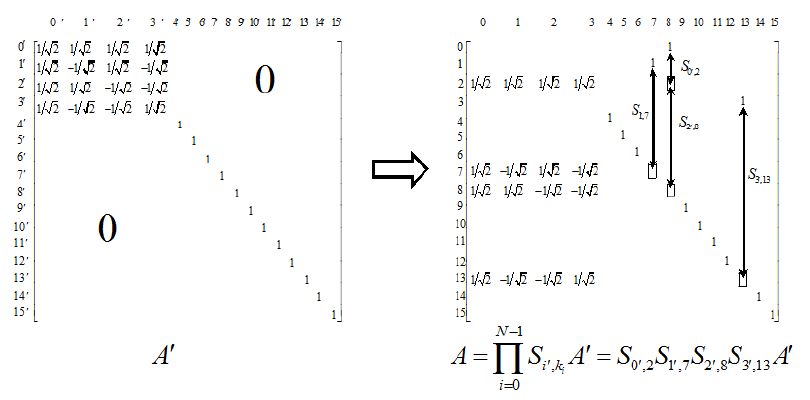
\includegraphics[width=\linewidth]{row_swap}
	\caption{Successive row swapping operations to transform $A'$ to $A$ in for the specific telephone database example. (credits to \cite{alsing2011grover})}
	\label{fig:row_swap}
\end{figure}

Calling $n$ the number of bits of the primary key (i.e. the contact \textit{name}) and $m$ the number of bits of the data field (i.e. the contact \textit{number}), the square matrix $A'$ will have a size of $K = 2^n \cdot 2^m = 2^{n+m}$ rows. Matrix $A'$ can be obtained as a direct sum $H^{\otimes n} \oplus I_{K-2^n}$ (see \cref{sec:direct_sum}).

Matrix $A$ can be obtained by applying to $A'$ a series of swap operators $S_{ij}$ that perform a swapping between rows $i$ and $j$ of a matrix. This operation is not described in the proposed paper, therefore we will try to give an algorithm to perform it (see \cref{sec:permutation}). This is the key passage that let us prepare an entangled register, ready to be used for the subsequent Grover iterations, as shown in the mentioned work.

\bigskip

This is a remarkable result, as it demonstrates the theoretical consistency of Grover's Algorithm for searching purposes. Critics can be raised against the performance or the convenience of the entire process with respect to the classical one, but these topics have already been discussed elsewhere \cite{1425397}.

\section{Permutation of rows in a matrix}
\label{sec:permutation}

The main issue that we want to address now is how to perform an arbitrary permutation of the rows of a ``quantum'' matrix. This is a fundamental algorithm passage for the correct implementation of Grover iteration. Despite that, we were not able to find any hint in literature on how to perform such permutations, so here we present some ideas that can be a starting point for a future improved and more general solution of the problem.

\bigskip

As it is well known in linear algebra, given a square matrix $M$ we can obtain $M'$ (a version of it where $i$-th and $j$-th rows are swapped) multiplying $M$ by a matrix $E$, where $E$ is the identity with $i$-th and $j$-th rows swapped:

\begin{equation*}
E M = M'
\end{equation*}
\begin{equation*}
	\begin{bmatrix}
	1 & 0 & 0 & 0\\
	0 & 1 & 0 & 0\\
	0 & 0 & 0 & 1\\
	0 & 0 & 1 & 0\\
	\end{bmatrix}
	\begin{bmatrix}
	a_{11} & a_{12} & a_{13} & a_{14}\\
	a_{21} & a_{22} & a_{23} & a_{24}\\
	a_{31} & a_{32} & a_{33} & a_{34}\\
	a_{41} & a_{42} & a_{43} & a_{44}\\
	\end{bmatrix}
	=
	\begin{bmatrix}
	a_{11} & a_{12} & a_{13} & a_{14}\\
	a_{21} & a_{22} & a_{23} & a_{24}\\
	a_{41} & a_{42} & a_{43} & a_{44}\\
	a_{31} & a_{32} & a_{33} & a_{34}\\
	\end{bmatrix}
\end{equation*}

\bigskip

Therefore our problem is to find a circuit that implements matrix $E$. This technique is consistent with the fact that a circuit applied on an array of qubit can be represented with a matrix multiplying the vector from the left side. Multiplying $E$ from the left of $M$ is equivalent to placing the circuit of $E$ after (on the right of) the circuit of $M$.

\begin{equation*}
\Qcircuit @R=1.0em @!R {
	\lstick{b_{0}: } & \multigate{2}{M}	& \multigate{2}{E}	& \qw \\
	\lstick{b_{1}: } & \ghost{M}		& \ghost{E}			& \qw \\
	\lstick{b_{2}: } & \ghost{M}		& \ghost{E}			& \qw \\
}
\end{equation*}

\subsection{Simplified case: 2 qubits}

If we have a circuit of only 2 qubits, swapping 2 rows can be relatively easy.

\bigskip

\noindent
\begin{tabular} {m{0.3\linewidth} m{0.7\linewidth}}
	\hline
	Rows to swap	& Matrices to apply\\
	\hline
	1, 2	&	ICNOT (\textit{NOT gate} controlled on first qubit = 0)\\
	1, 3	&	SWAP $\cdot$ ICNOT $\cdot$ SWAP\\
	1, 4	&	CNOT $\cdot$ SWAP $\cdot$ ICNOT $\cdot$ SWAP $\cdot$ CNOT\\
	2, 3	&	SWAP\\
	2, 4	&	CNOT $\cdot$ SWAP $\cdot$ CNOT\\
	3, 4	&	CNOT\\
	\hline
\end{tabular}

\bigskip

For example:

\begin{equation*}
CNOT \cdot SWAP \cdot CNOT = swap(2,4)
\end{equation*}
\begin{equation*}
\Qcircuit @R=1em @!R {
	\lstick{} & \ctrl{1}	& \qswap		& \ctrl{1}	& \qw \\
	\lstick{} & \targ	& \qswap \qwx	& \targ		& \qw \\
}
\end{equation*}

\begin{equation*}
\begin{bmatrix}
1 & 0 & 0 & 0 \\
0 & 1 & 0 & 0 \\
0 & 0 & 0 & 1 \\
0 & 0 & 1 & 0 \\
\end{bmatrix}
\begin{bmatrix}
1 & 0 & 0 & 0 \\
0 & 0 & 1 & 0 \\
0 & 1 & 0 & 0 \\
0 & 0 & 0 & 1 \\
\end{bmatrix}
\begin{bmatrix}
1 & 0 & 0 & 0 \\
0 & 1 & 0 & 0 \\
0 & 0 & 0 & 1 \\
0 & 0 & 1 & 0 \\
\end{bmatrix}
=
\begin{bmatrix}
1 & 0 & 0 & 0 \\
0 & 0 & 0 & 1 \\
0 & 0 & 1 & 0 \\
0 & 1 & 0 & 0 \\
\end{bmatrix}
\end{equation*}

\subsection{General case: shift and control}

A possible extension of the algorithm to the case of $n$ qubits would make an intensive use of controlled gates. Control through a qubit equal to 1 is equivalent to the direct sum of an identity matrix and the controlled gate itself. This means that, if we can control a gate, we are able to replicate the behavior of its $4 \times 4$ matrix in the bottom half of a larger $8 \times 8$ matrix (in terms of rows swapping). It could be interesting if we could temporarily ``move down'' the rows of a big matrix, perform our swaps and then move them up again. To easier describe this process we will make some definitions.

\bigskip

\textit{Definition.} Let $N$ denote the number of rows in the matrix representing an operation $G$. The number $N$ is obviously $2^n$, where $n$ is the number of bits on which gate $G$ is applied. Let's consider only a gate G which is decomposable as a direct product of a matrix $M$ and an identity matrix $I_k$. We will call $k$ the \textit{grade} of operator $G$.

\bigskip

Example:
\begin{itemize}
	\item CNOT and SWAP have \textit{grade} 0
	\item CNOT3, SWAP3 and SHIFT3 (\cref{sec:derived_gates}) have \textit{grade} 1
	\item SHIFT4 (\cref{sec:derived_gates}) has \textit{grade} 2
	\item CCNOT has grade 0
\end{itemize}

We can easily increase by $h$ the degree of a matrix $G$ by performing $kron(G, I_h)$. This is equivalent, in a register large $n+h$ qubits, to apply $G$ to the first $n$ qubits and nothing to the remaining $h$.

\subsubsection{Algorithm}

Let's take as an example the problem of permuting rows of an $8 \times 8$ matrix.

Using CNOT3, SWAP3 and ICNOT3 we can exchange matrix macroblocks (blocks of 2 contiguous lines). We can then operate on the two blocks (each 2x8) of the lower half-matrix using the CCNOT, CSWAP and controlled ICNOT ports, with granularity of the individual rows. Please note that the CSWAP allows us to exchange two rows of two different blocks (2x8), this can be useful in the generalization to more qubits. The same algorithm can be used for 16x16 matrices, increasing by one the degree of all previous ports and adding one more bit of control to the existing port (thus obtaining CCCNOT, CCICNOT, CCSWAP...).

Useful gates to perform the shift are SHIFT, QSD and QSU gates, together with their higher grade versions (\cref{sec:derived_gates}).

\subsubsection{Open issues}

Probably the addition of new control qubits at each step of generalization implies an exponential growth in spatial complexity of the circuit.

\subsection{General case: sorting algorithms}

This approach, instead of focusing on single row swaps, treats the permutation from initial to final matrix as a single process. You can see the analogy with sorting algorithms applied to arrays (bubble sort, merge sort...).

If there was a way to swap 2 consecutive rows of a matrix, regardless of their position, the problem would be easily solved. In that case we could apply bubble sort as an algorithm to rearrange all the rows as we like.

\bigskip

The only general way that we could devise to exchange consecutive rows is to use $X$ gates in direct sum with $I_2$ matrices all over the diagonal. The main drawback of this method is that this configuration is only able to swap rows $2i+1$ and $2i+2$, with $i \geq 0$. Therefore if we want to swap for example rows 2 and 3 we need to use a SWAP gate in direct sum with an appropriate number of $I$ matrices down the diagonal. The problem in using SWAP in this configuration is that it works only for swapping rows $4i+2$ and $4i+3$, with $i \geq 0$. Therefore if we want to swap rows 4 and 5 we need a new different gate (possibly $8 \times 8$ or bigger) and so on.

%\section{Feasibility analysis}

%TODO
	%!TEX root = main.tex

\begin{appendices}

\lstset{
	language=octave,
	basicstyle=\linespread{0.9}\ttfamily,		% line space
}

\chapter{Quantum gates in Octave}
\label{chp:octave}

Octave is a free software and a scientific programming language whose syntax is largely compatible with Matlab.

To fill the gap between some theoretical papers (which perform calculations on matrices) and quantum gates (that are eventually how those matrices are implemented) we modeled some quantum matrices as combination of known gates. In this way it was possible to investigate on how such matrices could be really implemented.

Therefore here we show the implementation of some gates used in other chapters.

\section{Elementary (existing) gates}

\subsection{Hadamard and X, Y, Z}

We will show only $H$ as an example, but the same applies for $X$, $Y$ and $Z$ and in general for $2 \times 2$ gates.

\noindent
\begin{tabular}{m{.5\linewidth} m{.5\linewidth}}
	Circuit	& Octave code\\
	\hline
	\begin{equation*}
	\Qcircuit @R=1em @!R {
		\lstick{b_{0}: } & \gate{H} & \qw \\
	}
	\end{equation*}
	&
	\begin{lstlisting}
	H = [
	1,  1; 
	1,  -1
	]./sqrt(2);
	\end{lstlisting}
\end{tabular}

\subsection{CNOT}

\noindent
\begin{tabular}{m{.5\linewidth} m{.5\linewidth}}
	Circuit	& Octave code\\
	\hline
	\begin{equation*}
	\Qcircuit @R=1em @!R {
		\lstick{b_{0}: } & \ctrl{1} & \qw \\
		\lstick{b_{1}: } & \targ    & \qw \\
	}
	\end{equation*}
	&
	\begin{lstlisting}
	CNOT = C(X);
	\end{lstlisting}
\end{tabular}

\subsection{ICNOT: inverted CNOT}

\noindent
\begin{tabular}{m{.5\linewidth} m{.5\linewidth}}
	Circuit	& Octave code\\
	\hline
	\begin{equation*}
	\Qcircuit @R=1em @!R {
		\lstick{b_{0}: } & \ctrlo{1} & \qw \\
		\lstick{b_{1}: } & \targ    & \qw \\
	}
	\end{equation*}
	&
	\begin{lstlisting}
	ICNOT = IC(X);
	\end{lstlisting}
\end{tabular}

\bigskip

Note that \textbf{it is not equivalent} to this circuit:

\noindent
\begin{tabular}{m{.5\linewidth} m{.5\linewidth}}
	\begin{equation*}
	\Qcircuit @R=1em @!R {
		\lstick{b_{0}: } & \targ     & \qw \\
		\lstick{b_{1}: } & \ctrl{-1} & \qw \\
	}
	\end{equation*}
	&
	\[
	\begin{bmatrix}
	1 & 0 & 0 & 0 \\
	0 & 0 & 0 & 1 \\
	0 & 0 & 1 & 0 \\
	0 & 1 & 0 & 0 \\
	\end{bmatrix}
	\]
\end{tabular}


\subsection{SWAP}

\noindent
\begin{tabular}{m{.5\linewidth} m{.5\linewidth}}
	Circuit	& Octave code\\
	\hline
	\begin{equation*}
	\Qcircuit @R=1em @!R {
		\lstick{b_{0}: } & \qswap      & \qw \\
		\lstick{b_{1}: } & \qswap \qwx & \qw \\
	}
	\end{equation*}
	&
	\begin{lstlisting}
	SWAP = [
	1, 0, 0, 0;
	0, 0, 1, 0;
	0, 1, 0, 0;
	0, 0, 0, 1;
	];
	\end{lstlisting}
\end{tabular}

\subsection{CCNOT}

\[
CCNOT =
\begin{bmatrix}
1 & 0 & 0 & 0 & 0 & 0 & 0 & 0\\
0 & 1 & 0 & 0 & 0 & 0 & 0 & 0\\
0 & 0 & 1 & 0 & 0 & 0 & 0 & 0\\
0 & 0 & 0 & 1 & 0 & 0 & 0 & 0\\
0 & 0 & 0 & 0 & 1 & 0 & 0 & 0\\
0 & 0 & 0 & 0 & 0 & 1 & 0 & 0\\
0 & 0 & 0 & 0 & 0 & 0 & 0 & 1\\
0 & 0 & 0 & 0 & 0 & 0 & 1 & 0\\
\end{bmatrix}
\]

\noindent
\begin{tabular}{m{.5\linewidth} m{.5\linewidth}}
	Circuit	& Octave code\\
	\hline
	\begin{equation*}
	\Qcircuit @R=1em @!R {
		\lstick{b_{0}: } & \ctrl{1} & \qw\\
		\lstick{b_{1}: } & \ctrl{1} & \qw\\
		\lstick{b_{2}: } & \targ    & \qw\\
	}
	\end{equation*}
	&
	\begin{lstlisting}
	CCNOT = C(CNOT);
	\end{lstlisting}
\end{tabular}

\subsection{CSWAP}

\[
CSWAP =
\begin{bmatrix}
1 & 0 & 0 & 0 & 0 & 0 & 0 & 0\\
0 & 1 & 0 & 0 & 0 & 0 & 0 & 0\\
0 & 0 & 1 & 0 & 0 & 0 & 0 & 0\\
0 & 0 & 0 & 1 & 0 & 0 & 0 & 0\\
0 & 0 & 0 & 0 & 1 & 0 & 0 & 0\\
0 & 0 & 0 & 0 & 0 & 0 & 1 & 0\\
0 & 0 & 0 & 0 & 0 & 1 & 0 & 0\\
0 & 0 & 0 & 0 & 0 & 0 & 0 & 1\\
\end{bmatrix}
\]

\noindent
\begin{tabular}{m{.5\linewidth} m{.5\linewidth}}
	Circuit	& Octave code\\
	\hline
	\begin{equation*}
	\Qcircuit @R=1em @!R {
		\lstick{b_{0}: } & \ctrl{1}    & \qw\\
		\lstick{b_{1}: } & \qswap      & \qw\\
		\lstick{b_{2}: } & \qswap \qwx & \qw\\
	}
	\end{equation*}
	&
	\begin{lstlisting}
	CSWAP = C(SWAP);
	\end{lstlisting}
\end{tabular}


\section{Operations between gates}

\subsection{Kronecker product (or direct product)}

\noindent
\begin{tabular}{m{.5\linewidth} m{.5\linewidth}}
	Circuit	& Octave code\\
	\hline
	\begin{equation*}
	\Qcircuit @R=1em @!R {
		\lstick{b_{0}: } & \gate{H} & \qw \\
		\lstick{b_{1}: } & \gate{H} & \qw \\
	}
	\end{equation*}
	&
	\begin{lstlisting}
	kron(H, H);
	\end{lstlisting}
	
\end{tabular}

\subsection{Gate control (direct sum)}

\noindent
\begin{tabular}{m{.4\linewidth} m{.6\linewidth}}
	Circuit	& Octave code\\
	\hline
	\begin{equation*}
	\Qcircuit @R=1em @!R {
		\lstick{b_{0}: } & \ctrl{1} & \qw \\
		\lstick{b_{1}: } & \gate{H} & \qw \\
	}
	\end{equation*}
	&
	\begin{lstlisting}
	function out = C(gate)
	size = rows(gate);
	out = blkdiag(eye(size), gate);
	endfunction;
	\end{lstlisting}\\
	\begin{equation*}
	\Qcircuit @R=1em @!R {
		\lstick{b_{0}: } & \ctrlo{1} & \qw \\
		\lstick{b_{1}: } & \gate{H} & \qw \\
	}
	\end{equation*}
	&
	\begin{lstlisting}
	function out = IC(gate)
	size = rows(gate);
	out = blkdiag(gate, eye(size));
	endfunction;
	\end{lstlisting}
\end{tabular}

\bigskip
\noindent
Note that CNOT is a ``controlled $X$''.

\section{New (derivated) gates}
\label{sec:derived_gates}

\subsection{DSWAP}

Performs a swap of the first 2 and the last 2 rows of the matrix, i.e. flips the least significative qubit.

\[
DSWAP =
\begin{bmatrix}
0 & 1 & 0 & 0 \\
1 & 0 & 0 & 0 \\
0 & 0 & 0 & 1 \\
0 & 0 & 1 & 0 \\
\end{bmatrix}
\]

\noindent
\begin{tabular}{m{.5\linewidth} m{.5\linewidth}}
	Circuit	& Octave code\\
	\hline
	\begin{equation*}
	\Qcircuit @R=1em @!R {
		\lstick{b_{0}: } & \qw      & \qw \\
		\lstick{b_{1}: } & \gate{X} & \qw \gategroup{1}{2}{2}{2}{1em}{--}
	}
	\end{equation*}
	&
	\begin{lstlisting}
	DSWAP = kron(eye(2), X);
	\end{lstlisting}
\end{tabular}

\subsection{SHIFT}
\label{sec:shigt_gate}

This gate shifts rows of half the size of the matrix, i.e. flips the most significative qubit.

\[
SHIFT =
\begin{bmatrix}
0 & 0 & 1 & 0 \\
0 & 0 & 0 & 1 \\
1 & 0 & 0 & 0 \\
0 & 1 & 0 & 0 \\
\end{bmatrix}
\]

\noindent
\begin{tabular}{m{.5\linewidth} m{.5\linewidth}}
	Circuit	& Octave code\\
	\hline
	\begin{equation*}
	\Qcircuit @R=1em @!R {
		\lstick{b_{0}: } & \gate{X} & \qw \\
		\lstick{b_{1}: } & \qw      & \qw \gategroup{1}{2}{2}{2}{1em}{--}
	}
	\end{equation*}
	&
	\begin{lstlisting}
	DSWAP = kron(X, eye(2));
	\end{lstlisting}
\end{tabular}

\subsection{QSD: Quarter Shift Down}
\label{sec:qsd_gate}

This gate shifts rows down of a quarter the matrix.

\[
QSD =
\begin{bmatrix}
0 & 0 & 0 & 1 \\
1 & 0 & 0 & 0 \\
0 & 1 & 0 & 0 \\
0 & 0 & 1 & 0 \\
\end{bmatrix}
\]

\noindent
\begin{tabular}{m{.5\linewidth} m{.5\linewidth}}
	Circuit	& Octave code\\
	\hline
	\begin{equation*}
	\Qcircuit @R=1em @!R {
		\lstick{b_{0}: } & \ctrl{1}	& \qswap	& \ctrlo{1} & \qw \\
		\lstick{b_{1}: } & \targ    & \qswap \qwx & \targ	& \qw \\
	}
	\end{equation*}
	&
	\begin{lstlisting}
	QSD = ICNOT*SWAP*CNOT;
	\end{lstlisting}
\end{tabular}

\subsection{QSU: Quarter Shift Up}
\label{sec:qsu_gate}

This gate shifts rows down of a quarter the matrix.

\[
QSU =
\begin{bmatrix}
0 & 1 & 0 & 0 \\
0 & 0 & 1 & 0 \\
0 & 0 & 0 & 1 \\
1 & 0 & 0 & 0 \\
\end{bmatrix}
\]

\noindent
\begin{tabular}{m{.5\linewidth} m{.5\linewidth}}
	Circuit	& Octave code\\
	\hline
	\begin{equation*}
	\Qcircuit @R=1em @!R {
		\lstick{b_{0}: } & \ctrlo{1}	& \qswap	& \ctrl{1} & \qw \\
		\lstick{b_{1}: } & \targ    & \qswap \qwx & \targ	& \qw \\
	}
	\end{equation*}
	&
	\begin{lstlisting}
	QSU = CNOT*SWAP*ICNOT;
	\end{lstlisting}
\end{tabular}

\subsection{CNOT3}

CNOT of grade 1. Please note that it is different from CCNOT.

\begin{equation*}
CNOT3 =
\begin{bmatrix}
1 & 0 & 0 & 0 & 0 & 0 & 0 & 0\\
0 & 1 & 0 & 0 & 0 & 0 & 0 & 0\\
0 & 0 & 1 & 0 & 0 & 0 & 0 & 0\\
0 & 0 & 0 & 1 & 0 & 0 & 0 & 0\\
0 & 0 & 0 & 0 & 0 & 0 & 1 & 0\\
0 & 0 & 0 & 0 & 0 & 0 & 0 & 1\\
0 & 0 & 0 & 0 & 1 & 0 & 0 & 0\\
0 & 0 & 0 & 0 & 0 & 1 & 0 & 0\\
\end{bmatrix}
\end{equation*}

\bigskip

\noindent
\begin{tabular}{m{.5\linewidth} m{.5\linewidth}}
	Circuit	& Octave code\\
	\hline
	\begin{equation*}
	\Qcircuit @R=1em @!R {
		\lstick{b_{0}: } & \multigate{1}{CNOT} & \qw \\
		\lstick{b_{1}: } & \ghost{CNOT}    & \qw \\
		\lstick{b_{2}: } & \qw      & \qw \gategroup{1}{2}{3}{2}{1em}{--}
	}
	\end{equation*}
	&
	\begin{lstlisting}
	CNOT3 = kron(CNOT, eye(2));
	\end{lstlisting}
\end{tabular}


\subsection{SWAP3}

\begin{equation*}
SWAP3 =
\begin{bmatrix}
1 & 0 & 0 & 0 & 0 & 0 & 0 & 0\\
0 & 1 & 0 & 0 & 0 & 0 & 0 & 0\\
0 & 0 & 0 & 0 & 1 & 0 & 0 & 0\\
0 & 0 & 0 & 0 & 0 & 1 & 0 & 0\\
0 & 0 & 1 & 0 & 0 & 0 & 0 & 0\\
0 & 0 & 0 & 1 & 0 & 0 & 0 & 0\\
0 & 0 & 0 & 0 & 0 & 0 & 1 & 0\\
0 & 0 & 0 & 0 & 0 & 0 & 0 & 1\\
\end{bmatrix}
\end{equation*}

\noindent
\begin{tabular}{m{.5\linewidth} m{.5\linewidth}}
	Circuit	& Octave code\\
	\hline
	\begin{equation*}
	\Qcircuit @R=1em @!R {
		\lstick{b_{0}: } & \qswap & \qw \\
		\lstick{b_{1}: } & \qswap \qwx    & \qw \\
		\lstick{b_{2}: } & \qw      & \qw \gategroup{1}{2}{3}{2}{1em}{--}
	}
	\end{equation*}
	&
	\begin{lstlisting}
	SWAP3 = kron(SWAP, eye(2));
	\end{lstlisting}
\end{tabular}


\subsection{SHIFT3}

\begin{equation*}
SHIFT3 =
\begin{bmatrix}
0 & 0 & 0 & 0 & 1 & 0 & 0 & 0\\
0 & 0 & 0 & 0 & 0 & 1 & 0 & 0\\
0 & 0 & 0 & 0 & 0 & 0 & 1 & 0\\
0 & 0 & 0 & 0 & 0 & 0 & 0 & 1\\
1 & 0 & 0 & 0 & 0 & 0 & 0 & 0\\
0 & 1 & 0 & 0 & 0 & 0 & 0 & 0\\
0 & 0 & 1 & 0 & 0 & 0 & 0 & 0\\
0 & 0 & 0 & 1 & 0 & 0 & 0 & 0\\
\end{bmatrix}
\end{equation*}

\subsubsection{Octave code}
\begin{lstlisting}
SHIFT3 = kron(SHIFT, eye(2));
\end{lstlisting}

\subsection{CNOT4}

CNOT of grade 2. Please note that it is different from CCCNOT.

\setcounter{MaxMatrixCols}{16}
\begin{equation*}
CNOT4 =
\begin{bmatrix}
\tikzmark{l1} 1 & 0 & 0 & 0 & 0 & 0 & 0 & 0 & 0 & 0 & 0 & 0 & 0 & 0 & 0 & 0\\
0 & 1 & 0 & 0 & 0 & 0 & 0 & 0 & 0 & 0 & 0 & 0 & 0 & 0 & 0 & 0\\
0 & 0 & 1 & 0 & 0 & 0 & 0 & 0 & 0 & 0 & 0 & 0 & 0 & 0 & 0 & 0\\
0 & 0 & 0 & 1 & 0 & 0 & 0 & 0 & 0 & 0 & 0 & 0 & 0 & 0 & 0 & 0\\
0 & 0 & 0 & 0 & 1 & 0 & 0 & 0 & 0 & 0 & 0 & 0 & 0 & 0 & 0 & 0\\
0 & 0 & 0 & 0 & 0 & 1 & 0 & 0 & 0 & 0 & 0 & 0 & 0 & 0 & 0 & 0\\
0 & 0 & 0 & 0 & 0 & 0 & 1 & 0 & 0 & 0 & 0 & 0 & 0 & 0 & 0 & 0\\
0 & 0 & 0 & 0 & 0 & 0 & 0 & 1\tikzmark{r1} & 0 & 0 & 0 & 0 & 0 & 0 & 0 & 0\\
0 & 0 & 0 & 0 & 0 & 0 & 0 & 0 & 0 & 0 & 0 & 0 & \tikzmark{l2}1 & 0 & 0 & 0\\
0 & 0 & 0 & 0 & 0 & 0 & 0 & 0 & 0 & 0 & 0 & 0 & 0 & 1 & 0 & 0\\
0 & 0 & 0 & 0 & 0 & 0 & 0 & 0 & 0 & 0 & 0 & 0 & 0 & 0 & 1 & 0\\
0 & 0 & 0 & 0 & 0 & 0 & 0 & 0 & 0 & 0 & 0 & 0 & 0 & 0 & 0 & 1\tikzmark{r2}\\
0 & 0 & 0 & 0 & 0 & 0 & 0 & 0 & \tikzmark{l3}1 & 0 & 0 & 0 & 0 & 0 & 0 & 0\\
0 & 0 & 0 & 0 & 0 & 0 & 0 & 0 & 0 & 1 & 0 & 0 & 0 & 0 & 0 & 0\\
0 & 0 & 0 & 0 & 0 & 0 & 0 & 0 & 0 & 0 & 1 & 0 & 0 & 0 & 0 & 0\\
0 & 0 & 0 & 0 & 0 & 0 & 0 & 0 & 0 & 0 & 0 & 1\tikzmark{r3} & 0 & 0 & 0 & 0\\
\end{bmatrix}
\end{equation*}
\DrawBox[thick, blue]{l1}{r1}{}
\DrawBox[thick, blue]{l2}{r2}{}
\DrawBox[thick, blue]{l3}{r3}{}


\noindent
\begin{tabular}{m{.5\linewidth} m{.5\linewidth}}
	Circuit	& Octave code\\
	\hline
	\begin{equation*}
	\Qcircuit @R=1em @!R {
		\lstick{b_{0}: } & \multigate{1}{CNOT} & \qw \\
		\lstick{b_{1}: } & \ghost{CNOT}    & \qw \\
		\lstick{b_{2}: } & \qw      & \qw\\
		\lstick{b_{2}: } & \qw      & \qw \gategroup{1}{2}{4}{2}{1em}{--}
	}
	\end{equation*}
	&
	\begin{lstlisting}
	CNOT4 = kron(CNOT, eye(4));
	\end{lstlisting}
\end{tabular}

\end{appendices}

	%!TEX root = main.tex

\chapter{Other ways explored during the research}
\label{chp:other}

Grover's Algorithm was originally devised to work with functions that are satisfied by a single input. Actually it has also been "generalized to search in the presence of multiple \textit{winners}". \cite{Boyer1998}

\bigskip

It turns out that Grover's Algorithm can be more useful in "speeding up the solution to NP-complete problems such as 3-SAT" than actual search. \cite{montanaro2016quantum}

\bigskip

We also considered spatial database search as a possible way of exploiting Grover's Algorithm, in the specific case of graphs with costs on arcs \cite{Aharonov:2001:QWG:380752.380758, childs2004spatial}.

Although there are some points of contact with Grover, none of them seemed to me of any use for our Max Flow Analysis problem.

%TODO
	%!TEX root = main.tex

\chapter{Conclusions}
\label{chp:conclusions}

In this work we explored several introductory aspects of quantum computing.

First of all Microsoft QDK, a quantum development environment that let us write programs for future quantum computers, and its language Q\#.

Then we got deep in the implementation of the entangled database for Grover Search, a specific part of the whole bigger algorithm that is often ignored and given for granted. In this context we provided not only a theory for performing passage needed to such entanglement, but also a working example of how this algorithm could be implemented with real gates.

Although the original purpose of this research project was to explore a new and unknown topic for the author, without any expectations, it turned out to be a little more. It was the opportunity to look with a critic eye to the state of the art and to propose approaches not yet explored, besides being of course a valuable experience.
	
	\bibliography{biblio}
	\bibliographystyle{abbrv}
	
\end{document}